%% This is an example first chapter.  You should put chapter/appendix that you
%% write into a separate file, and add a line \include{yourfilename} to
%% main.tex, where `yourfilename.tex' is the name of the chapter/appendix file.
%% You can process specific files by typing their names in at the 
%% \files=
%% prompt when you run the file main.tex through LaTeX.

\chapter{ChromoZoom v2: dynamic, online visualization of genomes and next-generation sequencing data}

\begin{marginfigure}[1cm]
  
\includegraphics[width=\textwidth]{chap3/chromozoom-gray}
  \emph{``The genome browser that lets you fly.''}
\end{marginfigure}

\begin{quote}
\emph{Although new sequencing technologies enable the automatic assembly of complete genomes from long reads and the generation of copious layers of functional data, sharing and collaboratively exploring these datasets remains difficult with current software. Genome browsers are the standard approach for interactively visualizing these data and may also facilitate collaboration if they are accessible via the web. The first version of ChromoZoom was written in 2012 as a fast, fluid web interface for genome browsing, although the design centered around scraped data for three reference genomes. With the present pace of \emph{de novo} assembly and resultant growth in the number of references, this strategy requires some rethinking. Here, we present a re-engineered version of ChromoZoom that can dynamically load custom genome assemblies and related data and also adds many new features that support pathogen surveillance activities at Mount Sinai.}
\end{quote}

\newthought{Genome browsers are indispensible} tools for modern experimental and computational biology. The size of typical genomic data (anywhere from tens of thousands of nucleotides for viruses into the billions for humans) prevents static plots from simultaneously capturing their scale and detail in a reasonable amount of space. Therefore, genome browsers are tasked with laying out the data in a way that is both interpretable and easily navigable. Most designs use a movable viewing region and map the contigs (in a completed assembly, the largest of which are the organism's chromosomes) to one axis of the coordinate system, usually a horizontal axis, while stacking the datasets onto the other axis. These other data can include range features such as genes and coding regions, continuous quantitative data like read depth and methylation levels, and mappings of other sequences, such as a different genome or the reads from a sequencing experiment. Many other datatypes exist and continue to be invented, but these are the basic shapes of data that genome browsers are now expected to handle.

Current genome browsers fall into three major categories, each with their own advantages and disadvantages. In fetching and drawing large amounts of heterogenous data, \emph{desktop-based browsers} like IGV,\autocite{Thorvaldsdottir2013} IGB,\autocite{Freese2016} and SmrtView\footnote{\url{https://github.com/PacificBiosciences/DevNet/wiki/SMRT-View}} have retained an advantage in being fastest during typical navigation operations, particularly when the data is being read from the user's local hard disk. All of the aforementioned desktop applications, however, use Java; this incurs the penalty of installing a Java VM in addition to the browser itself, and precludes their use on most mobile devices. Because of the need to the download software, these applications are not well-equipped for the rapid sharing of an active browsing session with a colleague, as website users are accustomed to doing by sending a URL or using ``share'' buttons. Nevertheless, they remain very popular for browsing large alignments from typical next-generation sequencing (NGS) experiments on humans and model organisms, since the size (and potential confidentiality) of these data often prevent them from being sent over the internet to web-based genome browsers. 

The first generation of web-based genome browsers like UCSC,\autocite{Dreszer2011} GBrowse,\autocite{Stein2002} Ensembl,\autocite{Stalker2004} and the NCBI Map Viewer\autocite{Wheeler2003} continue to retain the advantage of instant access from any web browser and the simplicity of sharing a particular view of the genome by linking to it. Since they were some of the first genome browsers to gain widespread use by wet lab biologists, and offered centralized repositories of valuable data during key moments of the birth of human genomics, they still tend to exhibit the widest array of well-curated data. UCSC's browser is well known for being the first to provide rapid, interactive access to early products of the Human Genome Project,\autocite{Kent2002} and remains prominent in human genomics for providing thousands of widely-used tracks that cover everything from tissue-specific expression and evolutionary conservation to clinically significant variants. However, since these software projects were built before modern web technologies like Asynchronous Javascript and XML (AJAX)\autocite{Paulson2005} and HTML5, the server must draw each user's data as an image that is sent to their browser, and the software's interactivity is therefore constrained compared to newer web applications. Unlike, e.g., Google Maps, none of these browsers allow the user to smoothly scroll, zoom, or ``throw'' the viewport (also called inertial scrolling), and they cannot draw new data without interrupting the user's movements. This latency makes it frustrating to gain an intuitive feel for distances or zoom levels and clashes with the experience users expect from the way scrolling\footnote{And pinching, since the release of the iPhone. Both operations on modern smartphones take pains to stay at a buttery smooth 60 frames per second, even if rendering quality has to be temporarily downgraded.} works on most other apps and websites.

A new generation of web-based genome browsers emerged around 2009 that embraced AJAX and employed JavaScript to draw data on the client-side. Of these, projects that have stayed active include JBrowse,\autocite{Buels2016} Dalliance,\autocite{Down2011} and Anno-J.\footnote{\url{http://www.annoj.org}} Among their advantages were a level of interactivity that approached the look and feel of the desktop-based browsers, without a need to download and install any software. Additionally, in some cases, views of the data could be shared as in the older web-based browsers. However, the new browsers were largely divorced from the core service of track curation that was integral to older web-based genome browsers, providing only barebones demo sites with a small number of sample tracks. Including the most recent entrants in this category, pileup.js\autocite{Vanderkam2016} and igv.js,\footnote{\url{https://github.com/igvteam/igv.js}} all of the next-generation genome browsers are primarily provided as source code libraries, which expect the users to install the code to their own web server and marry it to data via configuration or embedding of components within a larger website. Obviously, this reduces the accessibility of the software to teams with a web developer and a webserver.

There still is no genome browser that hits all the high marks of Google Maps in providing a (1) universally accessible, (2) richly interactive, and (3) easily sharable visualization of large, multilayered datasets. Without requiring any additional software, Google Maps even allows users to add custom data that is plotted on top of a map, and then share it via URL or embed it into another site.\footnote{An example of a running route in New York City: \url{https://goo.gl/GoHxx8}} Although Dalliance and JBrowse do offer some user interfaces (UIs) for layering and configuring user-provided tracks alongside server-provided data, they don't offer any sharing capabilities for these ``mashup'' views. In fact, none of the newer generation of web-based genome browsers emphasize this use case, assuming the involvement of a server administrator who can configure custom data sources. Finally, despite the increasing production of new genome layouts (or reference assemblies) as \emph{de novo} assembly of NGS data becomes commonplace, none of the new generation of web-based genome browsers allow a user to dynamically load a custom assembly (with annotation and sequence data) via their UI. Therefore, there are still avenues for improving web-based genome browsers to reach the level of the user experience that Google Maps first demonstrated possible in 2004 for geospatial data.\autocite{Vincent2007}

\section{Implementation}

The first version of ChromoZoom,\autocite{Pak2013a} released in 2012 at \url{http://chromozoom.org/}, attempted to achieve the three previously enumerated design goals, but targeted a small set of reference genomes in UCSC's database: GRCh37/hg19 (Human, Feb. 2009), NCBI36/hg18 (Human, Mar. 2006), and sacCer3 (Baker's yeast, Apr. 2011). At the time, we pursued a strategy of scraping UCSC's rendered images for these genome tracks at multiple zoom levels and serving them as tiles, similar to the approach of the first version of Google Maps.\footnote{See \textcite{Skinner2009}. Today, Google Maps renders all data using \href{https://developer.mozilla.org/en-US/docs/Web/API/WebGL_API}{WebGL} polygons when available, which allows for graphics processing unit (GPU) acceleration in the browser and high framerates.} Our approach ran into several roadblocks over time. Firstly, due to space constraints, it was impossible to scrape tiles for all of the thousands of tracks that UCSC hosts, so we had to focus only a small, frequently used subset for the two human assemblies. Secondly, since it was so computationally expensive to render all the tiles for a new genome, there was no expectation that the user could ever load a previously unseen genome assembly (or request that one be loaded) from the client side. Finally, the cost of re-rendering tiles made it difficult for us to keep tracks up to date with UCSC's data, even after we created our own local mirror of the UCSC genome browser. Although ChromoZoom did allow for user-provided custom data to be drawn alongside the tiled images using client-side JavaScript and \texttt{<canvas>} elements, we expected that server-hosted tracks would remain most popular.

As demand for viewing different genome assemblies and more varieties of custom data grew, we realized that our server-side tile scraping strategy would be untenable in the long run. Particularly in the context of pathogen surveillance and microbiology, where the number of completed reference genomes for certain species is already in the hundreds,\footnote{As of April 2017, there are 154 complete \emph{Staphyloccocus aureus} genomes on NCBI Genome: \url{https://www.ncbi.nlm.nih.gov/genome/genomes/154}} we discovered a general need for a web-based genome browser that could dynamically load a custom genome assembly with associated sequence, alignment, and annotation files. Although desktop-based genome browsers (particularly IGB) are able to open custom assemblies, their visualizations are not easily shared amongst a diverse team of wet lab biologists, bioinformaticians, and clinicians.

Therefore, we re-engineered ChromoZoom in its second release (v2) to support a new strategy of displaying every genome entirely via the use of \texttt{<canvas>} and scalable vector graphics (SVG), with client-side parsing and display of all contig layout, track annotation, and sequence data. The efficient fetching of track data that falls within the user's current viewport is facilitated by the use of bigBed and bigWig formats (big* formats),\autocite{Kent2010} which use binary compression that exceeds the storage efficiency of our previous tiled images (in PNG format). To test whether this new strategy scales, we scraped all active genomes from UCSC using a custom pipeline written in Python, which converts data from UCSC's MySQL database into bigBed formatted files or links directly to files hosted at UCSC that can be displayed directly by ChromoZoom. Heretofore we provide all UCSC genome data via this mechanism and not as tiled images.

ChromoZoom is still constructed as a single-page web application that implements most features in JavaScript, with heavy use of the jQuery UI library, and compilation into a single minified bundle using \texttt{browserify}.\footnote{\texttt{browserify} is \href{https://nodejs.org/}{node.js} package that can combine multiple JavaScript source files, including node modules, into a single bundle. See \url{http://browserify.org/}} All genomic data is fetched via AJAX from PHP scripts on the server that interface with libraries and utilities for each genomic data format, sometimes retrieving the backing data from another server.

For client-side performance, we continue to use tiled HTML5 elements that are rescaled and moved in accordance with user pan, zoom, and throw operations. We prerender into off-screen tiles to reduce loading latency and maintain a sense of location even when the viewport moves or zooms. For maximal performance when animating elements during viewport movement, we use the GreenSock Animation Platform.\footnote{GreenSock uses CSS3 transforms to enable hardware acceleration for most animations. See \url{https://greensock.com/}} To the greatest extent possible, fetching and parsing of annotation tracks and genome data occurs within Web Workers, which offload execution of JavaScript into processes that don't block the browser's main UI thread; this is a unique performance advantage of ChromoZoom over the other next-gen genome browsers.\autocite{Buels2016,Down2011,Vanderkam2016} Although most rendering is done in rasterized \texttt{<canvas>} tiles rather than vector graphics for performance reasons, we fully support high-DPI (i.e., ``retina'') displays by always rendering at the native pixel resolution of the display device.

\subsection{Availability}

ChromoZoom's source code is available from github at \url{https://github.com/rothlab/chromozoom}. ChromoZoom v2 can be viewed online by nearly any modern web browser (Chrome, Safari, Firefox, or IE11+) at \url{https://pakt01.u.hpc.mssm.edu/chromozoom/}, which will be also pushed to \url{http://chromozoom.org/} for its public release.

All source code is available under an AGPLv3 license\footnote{Briefly, this means that you can use ChromoZoom code for derivative web applications, as long those web applications are also open source. See \url{https://www.gnu.org/licenses/agpl-3.0.en.html}} and is free for academic and personal (but not commercial) use. For those that want to develop on the ChromoZoom codebase or deploy it locally (e.g., to view or serve data within a firewall), it can be installed to any Linux or macOS server with Apache web server, PHP 5.x, and a set of executables from \texttt{htslib} and Jim Kent's utilities, both of which are freely downloadable.\footnote{See \url{http://www.htslib.org/download/} and \url{http://hgdownload.cse.ucsc.edu/admin/exe/}.} Optionally, the user can also compile and install \texttt{bigBedSearch}, which is a separate software project created by the author\footnote{See \url{https://github.com/powerpak/bigBedSearch}} that adds better searching capabilities for bigBed formatted data.

\section{Results and Discussion}

\subsection{Data mirrored from UCSC}

183 genomes from UCSC were scraped for all track types compatible with ChromoZoom v2, which included bigWig, bigBed, BAM,\autocite{Li2009b} tabix-compressed VCF,\autocite{Danecek2011,Li2011} wiggle, and BED, and all track types readily convertible to the bigBed format, which included genePred, rmsk, PSL, GVF, and narrowPeak.\footnote{Descriptions of all formats used by UCSC can be found at \url{https://genome.ucsc.edu/FAQ/FAQformat.html}} This produced 8,702 converted bigBed files and 7,670 additional track entries that point directly to big* and BAM files on UCSC's servers. Collectively, the scraped tracks consume 485 GB of disk space. Since UCSC's MySQL database contains information on the update time for each table, we can re-run this process on a weekly schedule and only re-download data for tracks that have been updated, which occurs infrequently for almost all tracks. We therefore can efficiently keep our local bigBed files continuously synchronized with UCSC's database.

\subsection{Browsing a custom bacterial genome assembly}

Figure \ref{fig:bacterial_overall} provides an overview of the ChromoZoom v2 browser interface being used to visualize an assembled isolate of \emph{Staphyloccocus aureus} from The Mount Sinai Hospital.\footnote{The isolate was sequenced and assembled using the methods described in Chapter \ref{chap:steno}.} The interface uses the top line to display navigational controls, while the genome selection menu is in the lower right. This menu displays ``Custom Genome'' because the genome layout was not provided by the server, but was loaded directly from another source—in this case, an IGB Quickload Directory. Supported formats for custom genome assemblies will be covered later in this article.

\begin{figure*}[htb]
  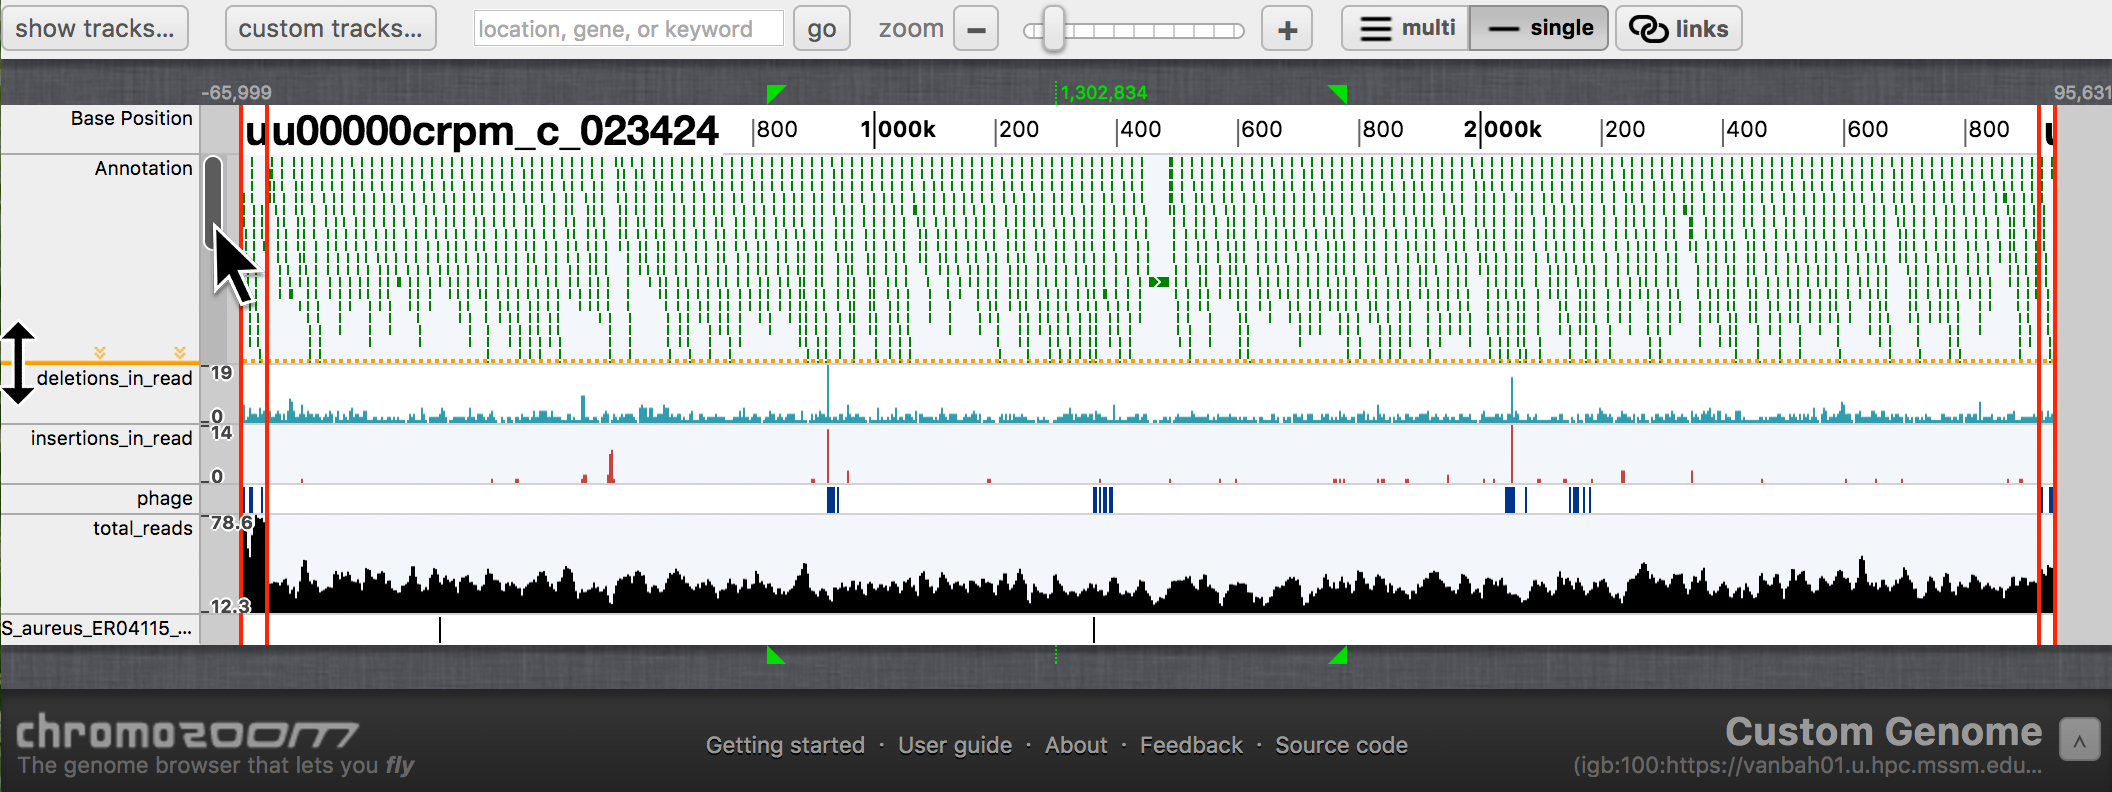
\includegraphics[width=\textwidth]{chap3/bacterial-ER04115}               
  \caption[Browsing a completed \emph{S. aureus} assembly with two plasmids]{Browsing a completed \emph{S. aureus} assembly with two plasmids (leftmost and rightmost small contigs). The top track, containing annotations of putative genes, has too much data to display in the available space (as is common for genomic data) which is indicated by the dotted orange line. This can be remedied by resizing the track (double arrow cursor) or scrolling (arrow cursor).}
  \label{fig:bacterial_overall}
\end{figure*}

Data is placed front and center in the main area of the interface. The user can click, drag, and throw this area horizontally to move. A green ``tank reticle'' is visible in the center of the screen, which helps provide feedback during zooming operations with the mousewheel (or two-finger scroll) and highlights the location that the user is zooming on. The display is at nearly the lowest zoom setting, so all three contigs are visible, and are separated by the bright red lines. The names of contigs are shown as the large labels in the ``Base Position'' track. Ticks in this track follow a minimalist format that avoids duplication of nonsignificant digits.\autocite{Krzywinski2013}

Six additional tracks are being displayed in this view, which are labeled along the left side of the tracks. The top track, in green, contains gene annotations by \texttt{prokka};\autocite{Seemann2014} this was supplied as a BED track. There are many such annotations in all contigs, and the orange dotted indicator below this track warns the user that some of the data is being clipped by the vertical space available. A scrollbar is available at the leftmost edge of the track to view the bottom edge of the track. 

The next two tracks in turquoise and red are bigWig tracks that count the number of deletions or insertions in reads, binned by base position. Two sharp peaks in the main chromosome that reach similar maximum values are notable (near the 900k and 2050k base positions), which happen to correspond with features in the next track, which contains putative phage regions.\footnote{This track was generated with \texttt{scripts/get\textunderscore repeats\textunderscore phage\textunderscore pai.py}, written by Mitchell Sullivan and incorporated into \href{https://github.com/powerpak/pathogendb-pipeline}{pathogendb-pipeline}.} These regions also appear to correlate with troughs in the depth of error-corrected reads, which is plotted on the subsequent ``total\textunderscore reads'' track. The last track shows single nucleotide variants (SNVs) created from a comparison using \texttt{nucmer} against a different but closely related hospital strain. Since there are only 2 SNVs separating these strains, they are related enough to consider that transmission (either between the patients or from a common source) was very likely.

\begin{marginfigure}
  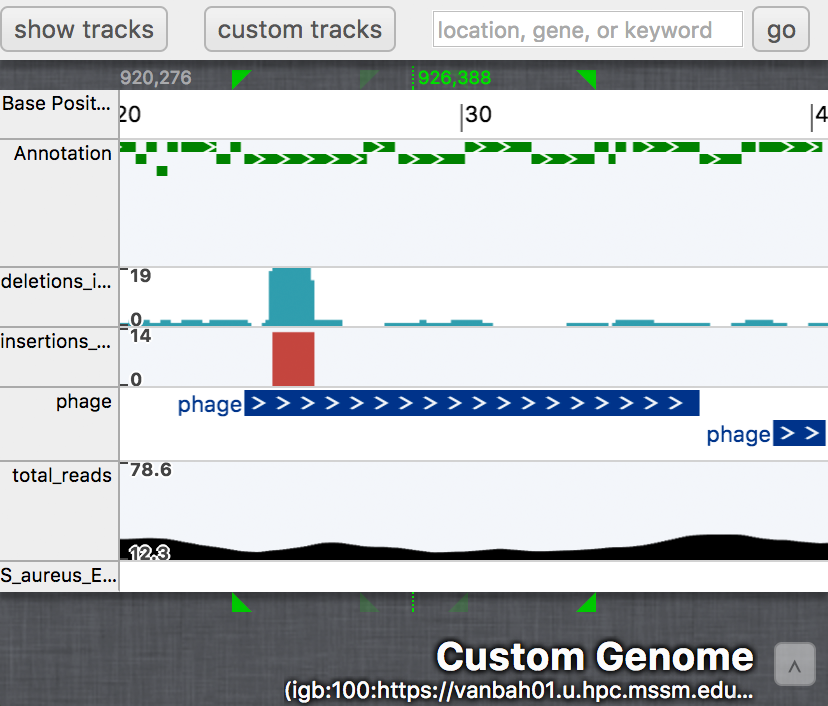
\includegraphics[width=\textwidth]{chap3/bacterial-phage}               
  \caption[A phage region corresponds to high insertion/deletion density]{A phage region corresponds to high insertion/deletion density.}
  \label{fig:bacterial_phage}
\end{marginfigure}

A zoomed view of the leftmost phage region in the large chromosomal contig is shown in Figure \ref{fig:bacterial_phage}. (This screenshot highlights the responsiveness of the top and bottom control bars to the resizing of the window: ChromoZoom is usable on displays as small as a smartphone screen.) This confirms that the peak in insertions and deletions is indeed in the middle of an annotated phage region and also a coding region annotated by \texttt{prokka}. An even closer look is depicted in Figure \ref{fig:bacterial_phage_variability}, which adds an alignment track (in BAM format) of the error-corrected reads created during the Hierarchical Genome Assembly Process.\sidecite[-1em]{Chin2013}
\begin{figure}
  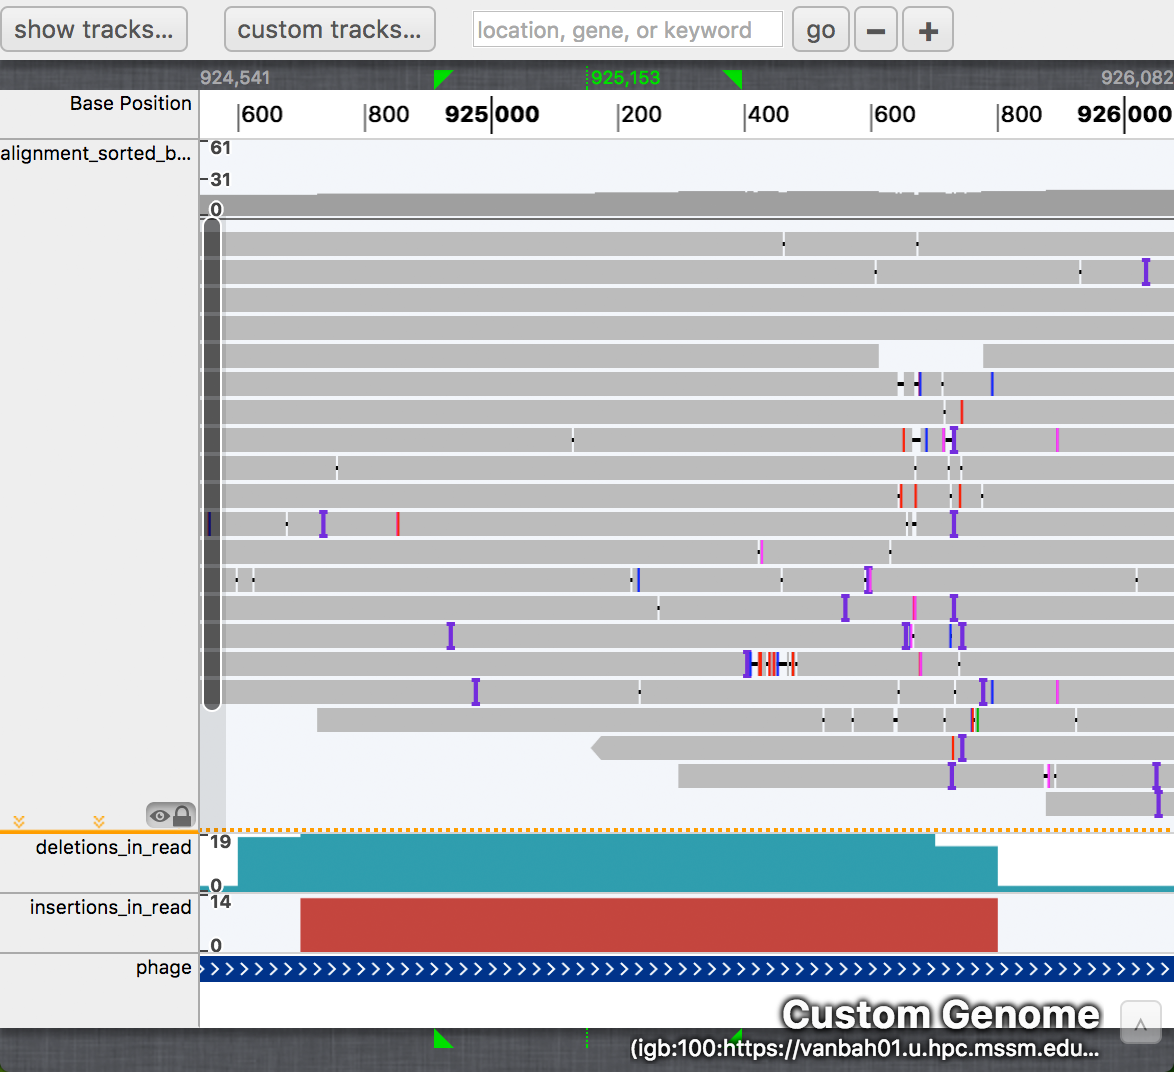
\includegraphics[width=\textwidth]{chap3/bacterial-phage-hypervariability}               
  \caption[Confirmation of a hypervariable region among phage genes]{Confirmation of a hypervariable region among phage genes. An alignment of error-corrected reads to the finished assembly has replaced the gene annotations as the top track, and it uses conventions for displaying BAM files that are similar to IGV. A coverage graph on the top of the track displays the depth of aligned reads, while the alignments themselves are displayed in a stack below, with notation symbols described in the main text. Judging from the totality of the evidence among all reads, the hypervariable region is approximately 200bp long and spans from 925,600 to 925,800.}
  \label{fig:bacterial_phage_variability}
\end{figure}
These alignments map the error-corrected reads back to the final contigs created during unguided assembly. The track uses display conventions similar to IGV:\autocite{Thorvaldsdottir2013} each aligned preassembled read is depicted as a gray block, with gaps relative to the reference shown as a horizontal black line, and insertions relative to the reference shown as the vertical purple I-bars. Single-base mismatches are depicted as colored vertical stripes in each read. From this view, it appears that an approximately 200bp region is particularly enriched for indels among the majority of the error-corrected reads, and therefore may represent a hypervariable region. Bacteriophages are known to contain genetic elements that generate diversity by site-directed, adenine-specific mutagenesis via reverse transcriptase-mediated exchange between two repeat sequences in order to alter their tropism and possibly also to evade the human immune system.\autocite{Liu2004,Minot2012} These sequences are relevant to pathogen surveillance because they potentially create inaccuracies in calculating genetic distances between bacterial strains, as they are expected to mutate faster than the remainder of bacterial DNA and therefore should be excluded when constructing phylogenies of hospital strains.

\begin{figure*}
  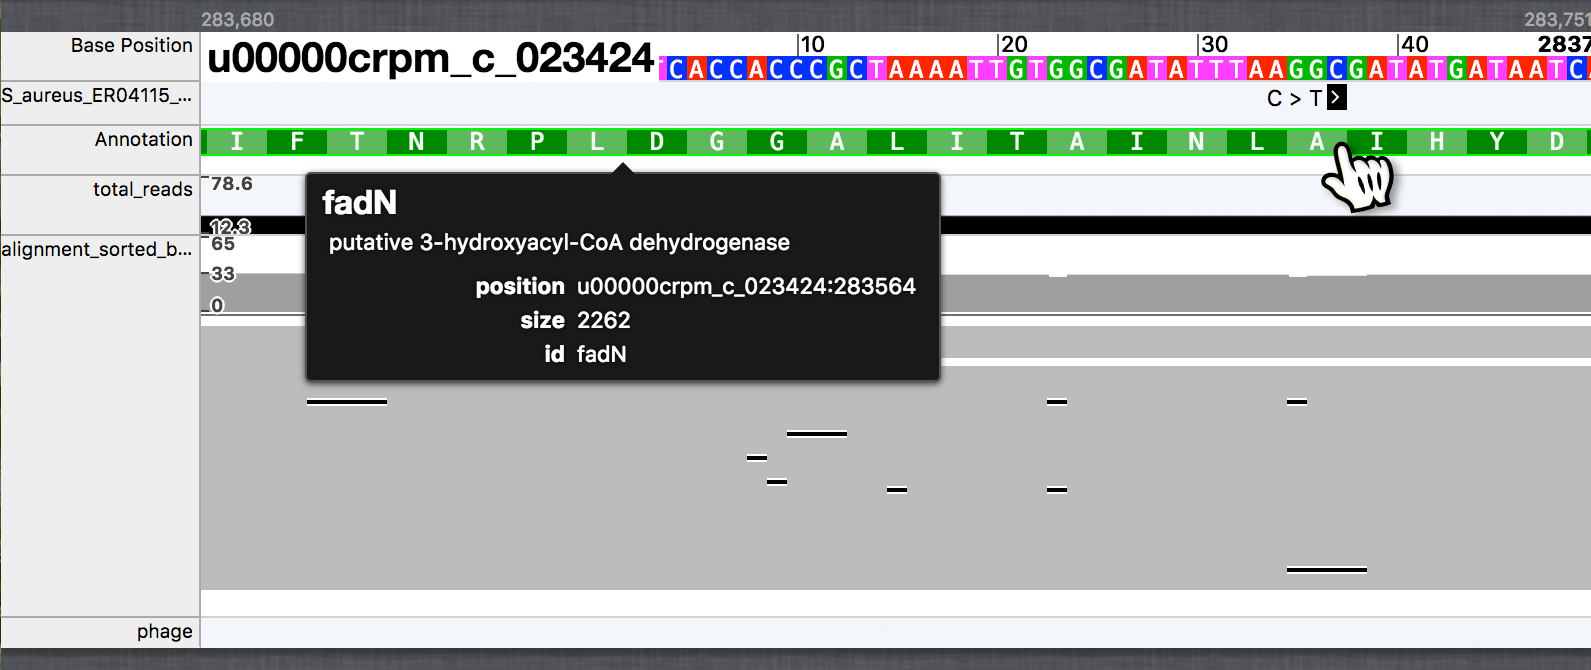
\includegraphics[width=\textwidth]{chap3/bacterial-snv}               
  \caption[A SNV between the two \emph{S. aureus} strains is in \emph{fadN}]{A SNV between the two \emph{S. aureus} strains is in \emph{fadN}, which putatively encodes a 3-hydroxyacyl-CoA dehydrogenase. Note that \emph{fadN} is on the negative strand while the SNV annotation (top track) is relative to the positive strand.}
  \label{fig:bacterial_snv}
\end{figure*}

When comparing two closely related bacterial strains from different patients or serial isolates from a single patient, as in Chapter \ref{chap:steno}, it can be revealing to examine the predicted effects of variants in protein-coding regions. These two particular isolates are from different patients and unrelated to a failure in antimicrobial therapy, so we might not expect any relationship between the SNV and antimicrobial resistance genes. The right-hand SNV seen in Figure \ref{fig:bacterial_overall} is in a phage region, and is therefore more likely a spurious variant call and unrelated to selective pressure on this strain. The left-hand SNV is not part of a phage region, however, and is shown in greater detail in Figure \ref{fig:bacterial_snv}. The surrounding region appears to have sufficient coverage by the error-corrected reads and shows generally consistent alignment among those reads.\footnote{After error correction of PacBio RSII reads, the most typical remaining errors are short indels, as seen above.} Therefore, this variant call likely reflects a true SNV, although for completeness, the locus for the corresponding SNV in the reverse direction should also be examined. The SNV is in a \emph{fadN} gene, whose homolog was previously identified in \emph{Bacillus subtilis} to be part of a 3-hydroxyacyl-CoA dehydrogenase/enoyl-CoA hydratase complex, which is involved in fatty acid degradation.\autocite{Matsuoka2007} This variant, which is aligned to the positive strand while the \emph{fadN} annotation is on the reverse strand, would cause a nonsynonymous Ala-697→Thr mutation. Since both isolates were cultured from separate, active infections, we can surmise that this mutation is probably not deleterious to fatty acid degradation in \emph{S. aureus}. (A more detailed functional analysis is beyond the scope of this article.)

This example shows that ChromoZoom v2 is able to quickly assess the quality and content of new bacterial genome assemblies and variant calls for related strains, which is crucial when infectious disease clinicians would expect to use these data as evidence for or against transmission, and the timeliness of potential interventions to prevent an outbreak is at stake. Because all data for this visualization was loaded from data accessible via the web, the URL for this view in ChromoZoom can be copied and pasted to easily share the visualization and its data with any member of the team, who can further explore it to their satisfaction. This allows labs and clinical groups to quickly collaborate on continuously shared NGS data from pathogens or any other newly sequenced organisms.

\subsection{Browsing NGS data for a human genome}

\begin{figure*}[htb]
  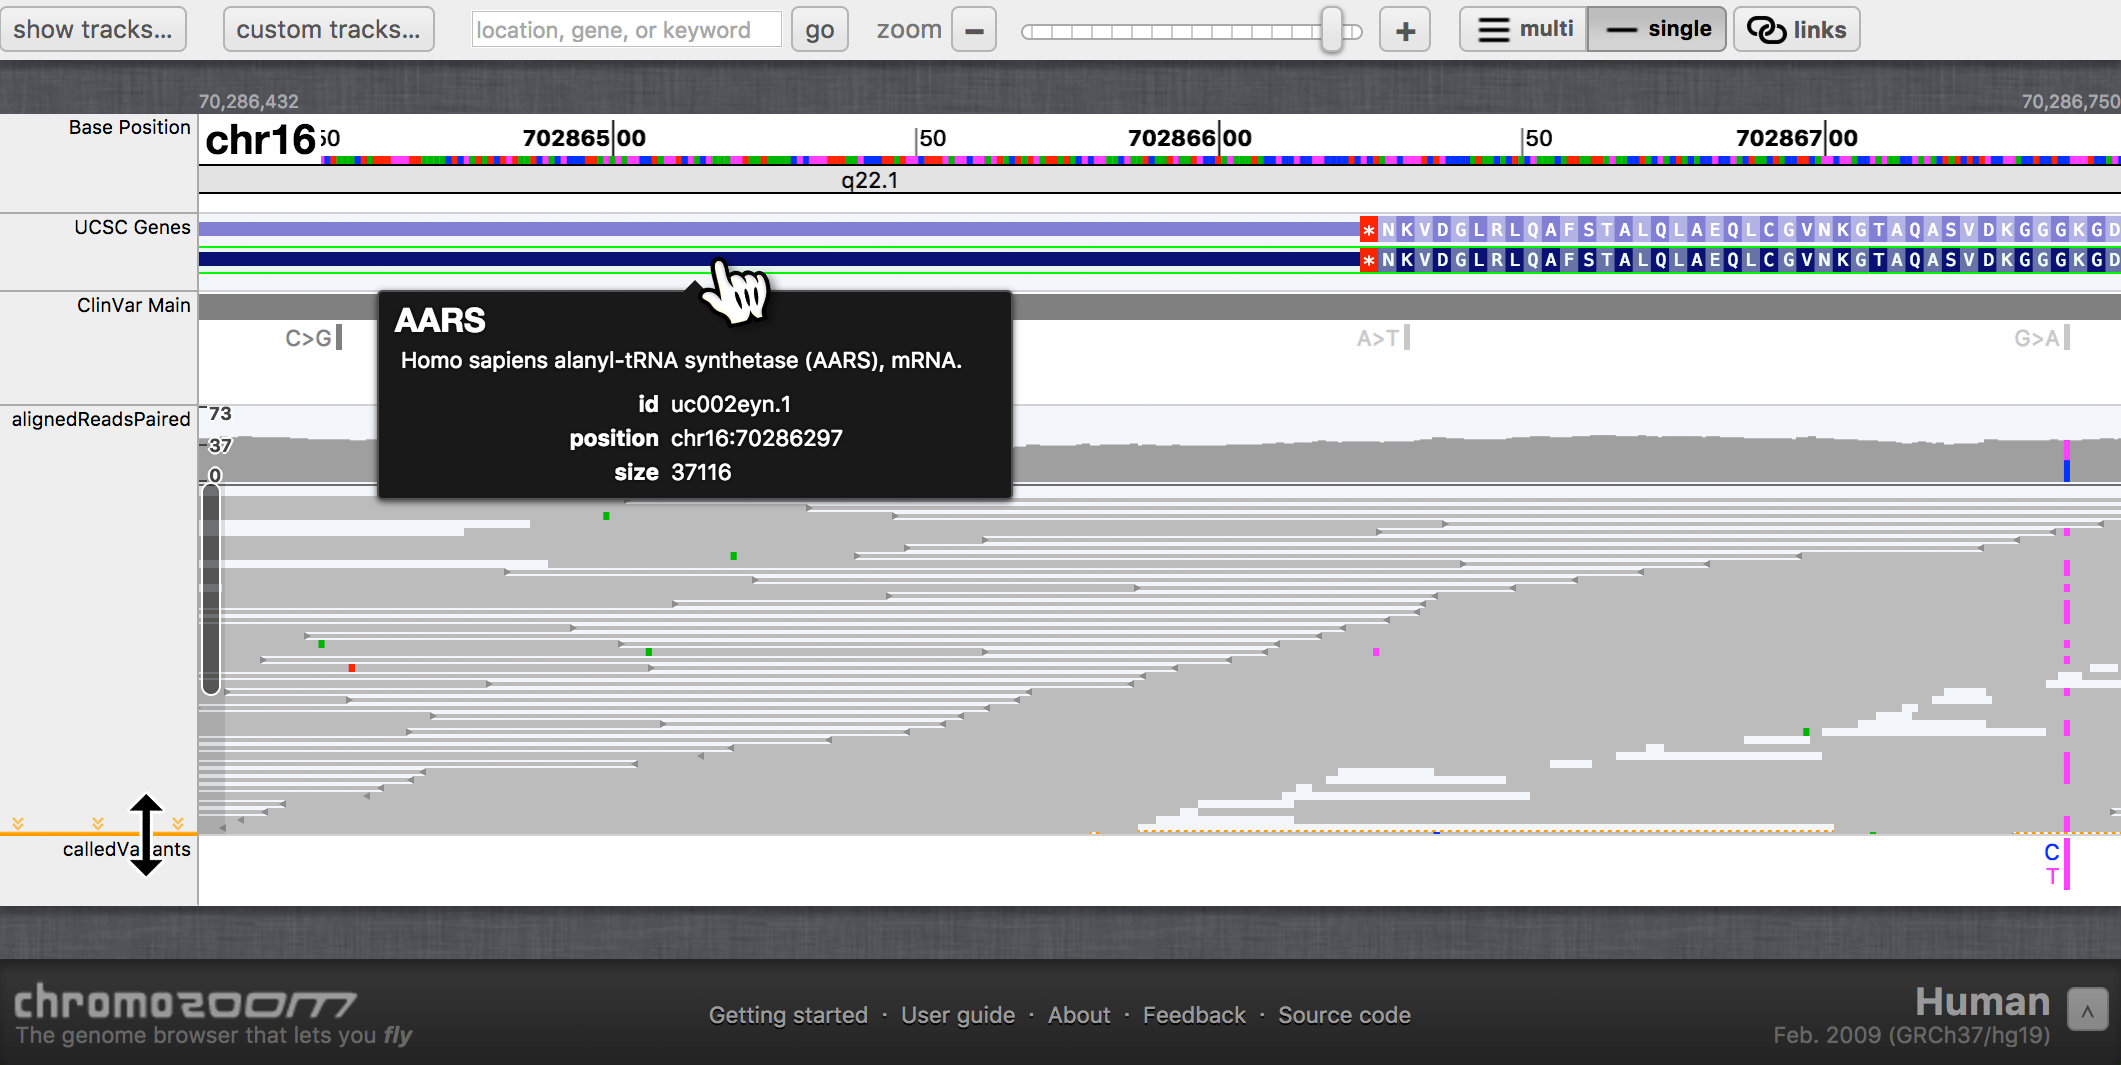
\includegraphics[width=\textwidth]{chap3/human-hg19}
  \vspace{-1em}
  \caption[NGS reads for the author's genome aligned to hg19]{\textbf{NGS reads for the author's genome aligned to hg19}, displayed in paired mode, and corresponding variant calls. The ``UCSC Genes'' and ``ClinVar Main'' tracks are mirrored from UCSC, while the other two were loaded from URLs pasted into the interface by the user; ``alignedReadsPaired'' is in BAM format while ``calledVariants'' is a tabix-compressed VCF file. A heterozygous C/T variant in the \emph{AARS} coding sequence is visible to the righthand side, which is annotated in the ClinVar track as a benign variant (light gray G>A; annotated to reverse strand). More alignments are stacked vertically than can be displayed, as indicated by the orange clipping indicator, which could be remedied by resizing the tracks or using the adjacent scrollbar (mouse cursors).\vspace{1em}}
  \label{fig:human-hg19}
\end{figure*}

ChromoZoom v2 is equally adept at browsing NGS data aligned to human and or other vertebrate references, which is a common task for both research and clinical diagnostic laboratories. Figure \ref{fig:human-hg19} depicts a ChromoZoom v2 visualization of NGS reads for the author's genomic DNA
generated as part of the Practical Analysis of a Personal Genome class offered at Mount Sinai.\autocite{Linderman2015} Sequencing was performed to approximately 30-fold mean coverage on an Illumina HiSeq using a 100bp paired-end protocol. Adding BAM files (with alignments) and tabix-compressed VCF tracks (containing variants)—both standard products of current NGS pipelines—can be performed by end users by clicking the ``custom tracks...'' button in the top toolbar and pasting URLs for the data. BAM files can be displayed in both single-end and paired-end mode.

As described in Implementation, for all of UCSC's active reference genomes, we utilized a track scraper to pull links to all supported track types in UCSC's MySQL database (with local conversion to the bigBed format as necessary), which gives ChromoZoom users quick access to a total of 7,969 UCSC-curated tracks for the hg19 reference. Clicking items in these tracks (such as the \emph{AARS} gene in Figure \ref{fig:human-hg19}) takes the user to corresponding item details page in UCSC.

With so many available tracks, searching and selecting interesting annotation sources can be challenging task for the UI to accomodate without overwhelming the user. ChromoZoom v2 uses the streamlined approach of a searchable, expandable list of tracks organized in the same hierarchy used by UCSC (Figure \ref{fig:track-search}). In this UI, we encourage discoverability by limiting the initial list to 11 expandable categories, with no more than 20 track and track groups inside each category. For the track groups, indicated by the left-hand arrows, the user can ``drill down'' into subtracks by expanding the hierarchy similar to the folder-tree views in most file managers. If the user is interested in a particular keyword, like ``kidney,'' they can start typing it, and this pulls all relevant subtracks to the forefront of the hierarchy and also filters the list only show tracks that at least partially match the query (Figure \ref{fig:track-search}). Once the user sees tracks that are potentially interesting, adding the data to the browser view is as simple as clicking a checkbox.

\begin{marginfigure}[-2.7cm]
  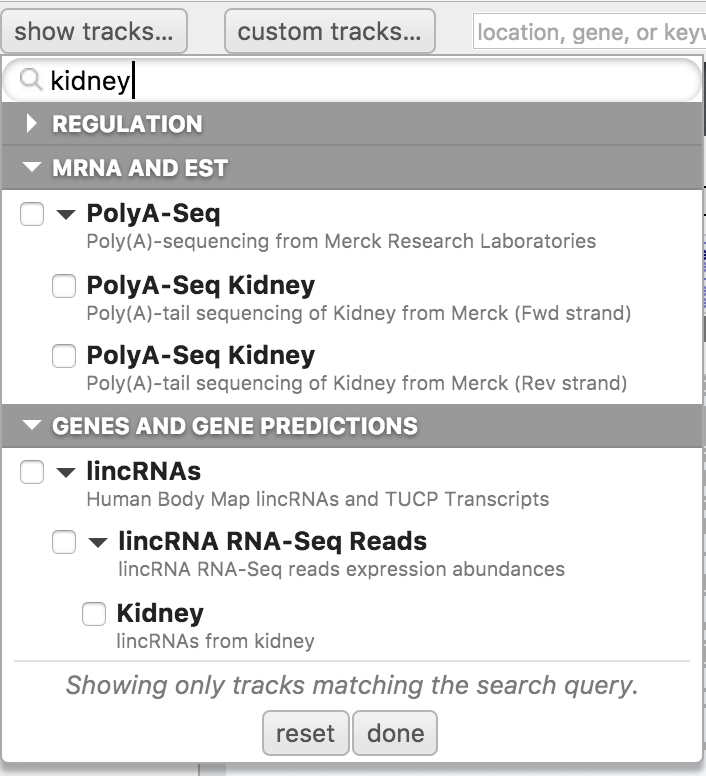
\includegraphics[width=\textwidth]{chap3/track-search}               
  \caption[Track searching interface for UCSC reference genomes.]{A searchable track interface allows quick discovery of relevant tracks from the thousands of tables available from UCSC, each of which can be added with a single click.}
  \label{fig:track-search}
\end{marginfigure}

Searching for features within tracks is equally necessary for fast navigation and is depicted in Figure \ref{fig:gene-search}. For all feature data scraped from UCSC's database, we make use of B-tree indices that can be added to the end of the bigBed formatted tracks that are saved to our server. These indices were added to the bigBed format specification after its first version was published,\autocite{Kent2010} but can now be easily created using the \texttt{-extraIndex} option of the \texttt{bedToBigBed} program from Jim Kent's utilities. B-trees allow fast prefix-based searching of prespecified fields in large tracks (even with millions of elements), which we automatically perform on UCSC tracks for fields like feature names and IDs. Searching is as easy as typing in the search box at the top of the browser, which immediately provides suggested results as the user types (similar to autocomplete on smartphones or Google Suggest).\footnote{Google Suggest was rolled out to the homepage of Google in 2008. See \url{https://goo.gl/2O53MP}} Using the search box, users can quickly jump to locations by chromosome coordinates, gene name, or other feature ID. For UCSC genomes, the default gene track is always included in searches, but any other tracks that are currently active will also be automatically searched too (Figure \ref{fig:gene-search}).

\begin{marginfigure}
  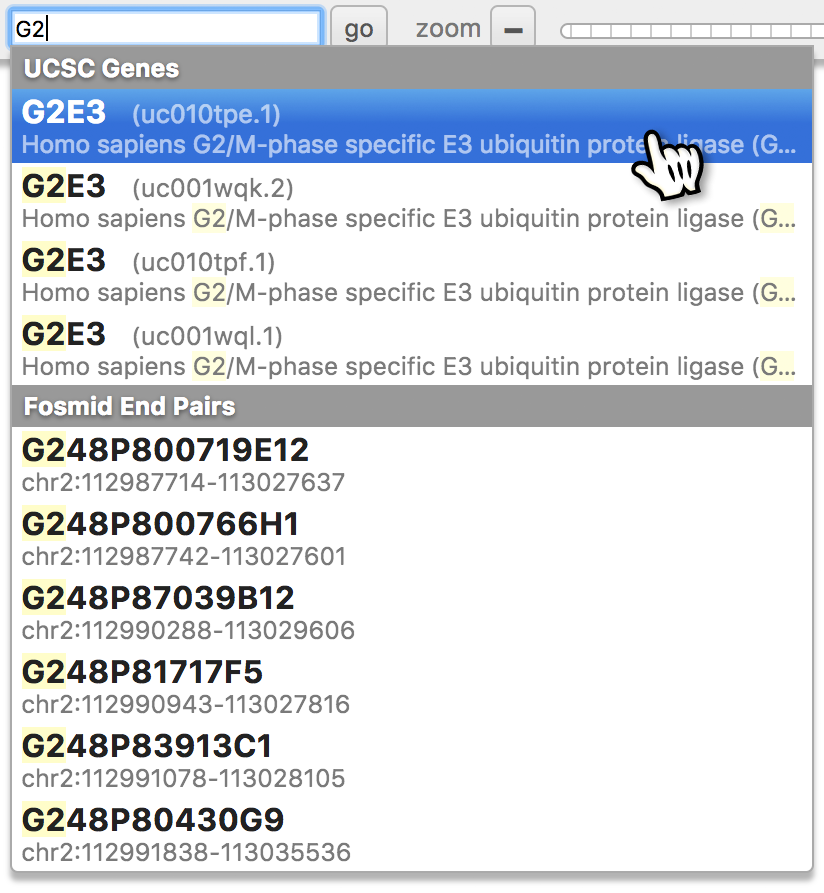
\includegraphics[width=\textwidth]{chap3/gene-and-fosmid-search}               
  \caption[Searching for features by name]{On all UCSC reference genomes, the primary gene track will be prefix-searched by name or ID. Also, any visible annotation tracks will be prefix-searched. In this example, the ``Fosmid End Pairs'' track (which catalogs all valid pairs of fosmid end sequences) was active, and therefore its items are also included in the search results. Results can be navigated by mouse and keyboard. Selecting a result will jump to its position in the browser.}
  \label{fig:gene-search}
\end{marginfigure}

\begin{figure*}[tbp]
  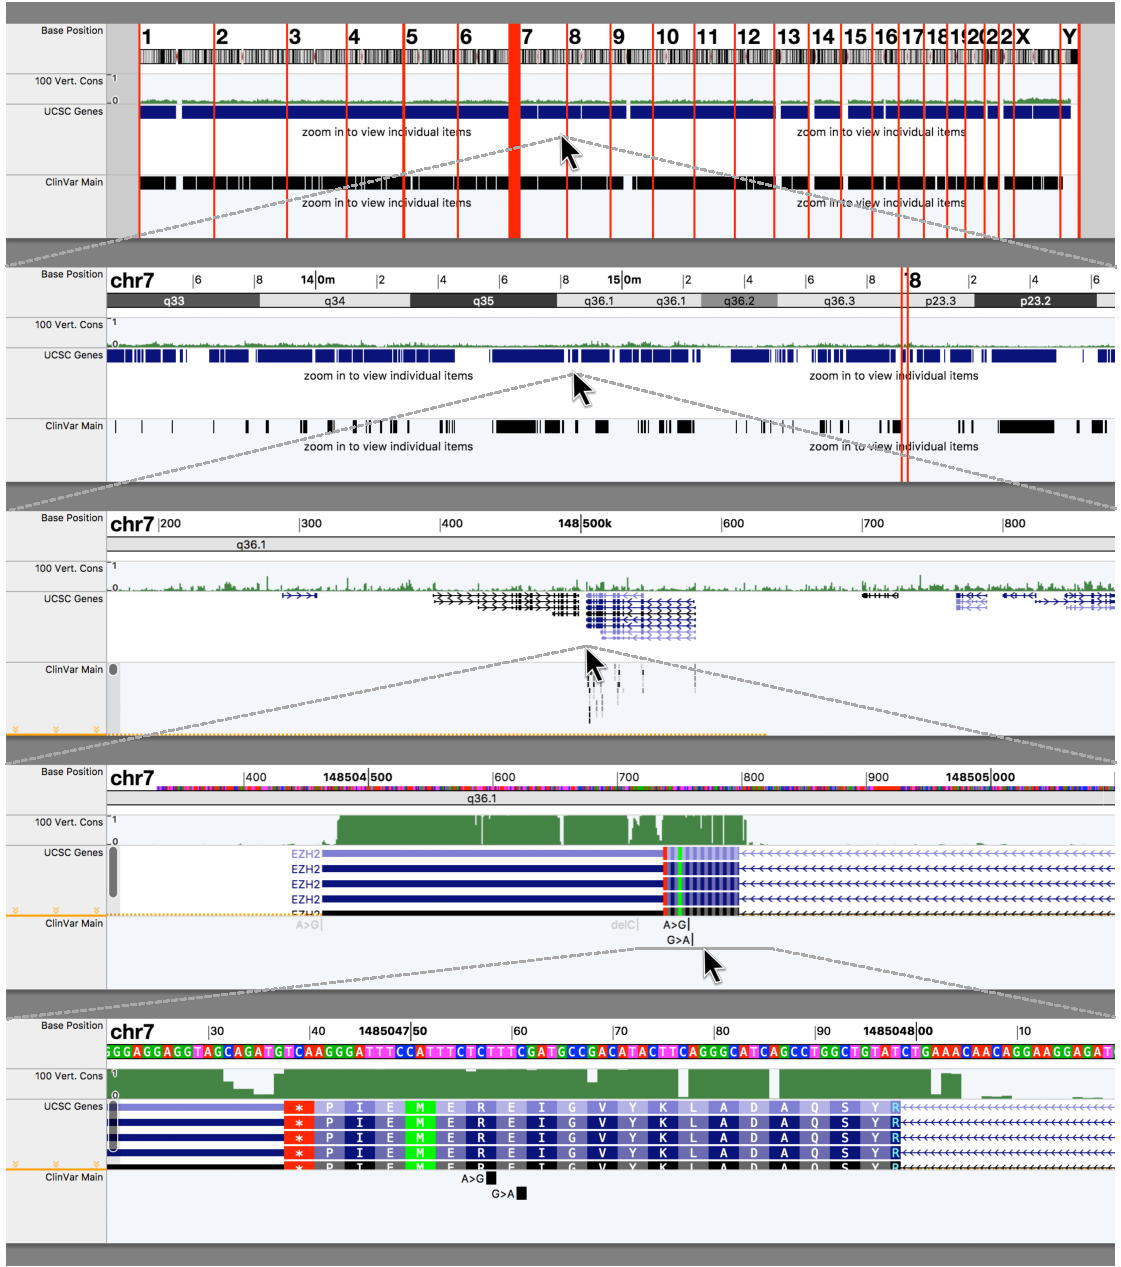
\includegraphics[width=0.9\textwidth,height=17cm,keepaspectratio]{chap3/human-hg19-weaver-cursors}       
  \fullwidthlabelcaption{fig:human-hg19-weaver}{ChromoZoom dynamically redraws ticks and tracks}{
    \textbf{ChromoZoom dynamically redraws ticks, ideograms, and tracks to suit the user's current track heights and zoom level.} The above shows a series of progressive zoom operations on three UCSC-curated tracks for the hg19 reference genome, starting from a view of all chromosomes and contigs and moving in towards a view of two specific variants within the \emph{EZH2} gene. The top track displays base position and ideogram bands, which are automatically overdrawn with nucleotide data as the user zooms. A green bigWig track displaying evolutionary conservation across 100 vertebrates is immediately underneath, followed by UCSC's gene track (dark blue) and the same uncolored ClinVar track seen in Figure \ref{fig:human-hg19}. Mousing over the variants in the bottom view reveals that they are both pathogenic and associated with Weaver syndrome.
  }
\end{figure*}

On genomes at the scale of the human reference assemblies, particularly when the data for each track potentially needs to be fetched from different servers, it is crucial for genome browsers to detect and gracefully handle cases when the user is viewing a region that has more data than can be fetched in a reasonable amount of time. Otherwise, as often occurs in other next-gen genome browsers, the initiation of a ``too-large'' data request will stall drawing of data interminably, cause the UI to become unresponsive, or in the worst case, crash the user's web browser. IGV and UCSC are generally smart enough to handle these cases, e.g., in IGV any region in a BAM file that contains too many reads is automatically downsampled. For ChromoZoom v2, in the case of bigBed, BAM, and tabix compressed formats, we perform an estimate of the average feature density that is calculated when the track is first loaded into the browser, and use that to estimate the optimal width of a range request. This width is then used for all requests, with the returned data cached in an intermediate layer (a \texttt{RemoteTrack} object) to avoid unnecessary refetching of any region. If the user is attempting to display a region size for which fetching item-level data is impractical, a summary of the data is requested instead, such as the positions covered by at least one item. Figure \ref{fig:human-hg19-weaver} shows this in action for the two lowest zoom levels on the ``UCSC Genes'' and ``ClinVar Main'' tracks, which have enough vertical space to start stacking features, but instead inform the user that they should ``zoom in to view individual items.'' As the user passes the estimated threshold for practical viewing of individual data, ChromoZoom automatically begins fetching and drawing them (bottom three rows of Figure \ref{fig:human-hg19-weaver}).

This is related to a similar ability that most current genome browsers lack, which is to always try to draw data at a detail level that is amenable to its quantity and the available space. Although in certain cases UCSC and IGV can adjust their drawing styles automatically, in most cases, they expect users to choose a style for each track from the rather obtuse menu of ``dense,'' ``squish,'' and ``pack.'' By and large, the approach of laying this choice on the user has carried over into next-gen genome browsers.\footnote{igv.js, \textcite{Buels2016,Down2011,Vanderkam2016}} By contrast, Google Maps and other online mapping websites have always applied cartographic principles in condensing and simplifying features to suit the map's scale, so that, e.g., at the world level only country borders and terrain are visible, while at the street level, individual buildings, transit stops, and business labels are visible—and this all occurs automatically while zooming. ChromoZoom adopts this approach, and whenever the user zooms it automatically adjusts its drawing styles to best fit the data to the viewport for each track, including the automatic addition of codons and individual nucleotides at the closest scales (Figure \ref{fig:human-hg19-weaver}). If this algorithm isn't providing as much detail as the user needs, perhaps because the user wants to examine or click individual items even when they can't all fit on the screen, the user is always able activate the most detailed display available by using a single button in the sidebar (Figure \ref{fig:eye-lock}).

\begin{marginfigure}
  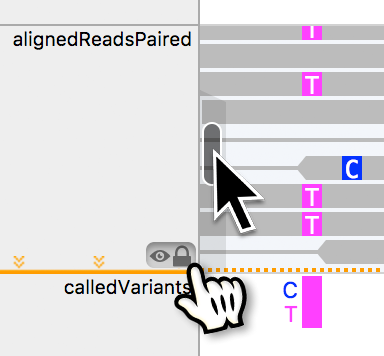
\includegraphics[width=\textwidth]{chap3/eye-lock}               
  \caption[Forcing the most detailed display mode]{If users need to see individual items even if there are too many to fit vertically, there is an ``eye-lock'' button in the bottom right corner of each track's sidebar (hand cursor). This forces the display of individual items, if possible, and then the user can then scroll vertically as needed with the scrollbar (arrow cursor).}
  \label{fig:eye-lock}
\end{marginfigure}

Most importantly, ChromoZoom takes great care to maintain immersion in the ``landscape'' of genome features as the user zooms through all levels, using animation of the UI during zoom and redraw operations to keep continuity between all the rendered items even if details are added or removed. These animations can't be depicted in Figure \ref{fig:human-hg19-weaver}, but they are central to the design of ChromoZoom and therefore are generally achieved with better fidelity than in other web-based genome browsers, which typically have to display spinners or change the layout of onscreen items during jarring pauses.

As seen above, ChromoZoom v2 offers powerful features for the interactive display of NGS data on top of standard vertebrate references, and is useful for placing the typical outputs of NGS pipelines (like BAM and VCF data) in the context of thousands of rich annotations from UCSC's databases.

\subsection{Supported genome formats}

Using the genome picker in the bottom right of the screen, users are able to change the currently displayed genome assembly to others available from UCSC, or load their own in several formats supported by ChromoZoom. These formats currently are: FASTA files, which only contain contigs and sequence data in plain text; GenBank files, which contain contigs, sequence data and annotations in plain text; \texttt{chrom.sizes} files, which are lists of contigs and their lengths that do not contain any sequence data; and IGB Quickload directories, which can contain a contig layout, sequence data, and both binary and plaintext annotation data. Of these formats, the first three (FASTA, GenBank, and \texttt{chrom.sizes}) can be read directly from the user's hard disk, pasted from the clipboard, or fetched via URL.

IGB Quickload Directories cannot be read directly and must be uploaded somewhere on the web for usage with ChromoZoom, so they require additonal setup compared to the other formats. However, they are also the most feature-rich, as the user is able to customize the display of any number of annotation tracks in any format. The \emph{S. aureus} genome displayed in Figures \ref{fig:bacterial_overall}-\ref{fig:bacterial_snv} was provided to ChromoZoom as an IGB Quickload Directory, and it contained a mixture of BAM, BED, and bigWig tracks, along with sequence data in the form of a \texttt{.2bit} file.\footnote{TwoBit sequence is a standard format created by UCSC and is described at \url{https://genome.ucsc.edu/goldenpath/help/twoBit.html}. It is a binary format that is more compact than FASTA, and can be created from FASTA files using the \texttt{faToTwoBit} executable in Jim Kent's utilities.} As the name suggests, the Quickload format was developed as a way to easily load annotated genomes into IGB. We retain complete compatibility with IGB's specifications so either program can open the same files, and full instructions for creating a directory is available in IGB's documentation.\footnote{See \url{https://wiki.transvar.org/display/igbman/Sharing+data+using+QuickLoad+sites}} Briefly, a minimal directory should include a \texttt{.2bit} file with the sequence data, a plaintext \texttt{genome.txt} file (that can be generated from the \texttt{.2bit} file) listing all contigs and their sizes in the preferred order, and an \texttt{annots.xml} file that specifies the annotation tracks that should be loaded alongside the genome.

\subsection{Supported track formats}

ChromoZoom v2 retains support for a diverse array of annotation track formats, and due to its new design of loading all data from these files rather than a backend database or cached image tiles, all of these formats are handled equally whether supplied by the server or by the client. Plaintext formats are the easiest for users to edit by hand or generate from spreadsheet programs, and remain appropriate for data that can be uploaded or downloaded in their entirety in a reasonable amount of time (likely becoming somewhat slow at around \textasciitilde{}10MB).\footnote{Because plaintext files don't include any indexes, the whole file must be obtained before any data can be displayed.} For interval-based features, such as gene predictions or alignments, we support the BED format defined by UCSC, including the use of arbitrary fields at the right end of each line (sometimes called BED plus or BED extra fields),\footnote{This requires the use of a track line that lists the extra fields' names as a comma-separated list in the \texttt{bedPlusFields} option.} and we also parse the standard \texttt{FEATURES} section of any GenBank files loaded as a custom genome. For continuous quantitative data, both bedGraph and WIG are supported, again using UCSC's specifications.

Binary formats are generally preferable because they allow for indexing and partial loading from remote locations via the use of HTTP \texttt{Range:} requests,\autocite{Li2009b,Li2011a,Kent2010} although they do require slightly more setup and need to be uploaded somewhere on the web to work with ChromoZoom. We support bigBed files for interval features, BAM files for alignments, bigWig files for continuous quantitative data, and tabix-compressed VCF files for variant calls. URLs pointing to any of these filetypes can be pasted into ChromoZoom and they will display alongside the currently loaded reference.\footnote{We don't support the direct uploaad of these files, because they can easily exceed 100GB each and therefore would be impractical to transfer and store. We do intend to support opening files directly from users' Dropbox accounts, however—coming soon!} These are also the same file types now used to display all data for the UCSC reference genomes. bigBed files may include extra fields in extra columns similarly to BED files, which ChromoZoom uses to display expanded tooltips containing the customized per-item information that UCSC has on most of their curated tracks.

\begin{marginfigure}
  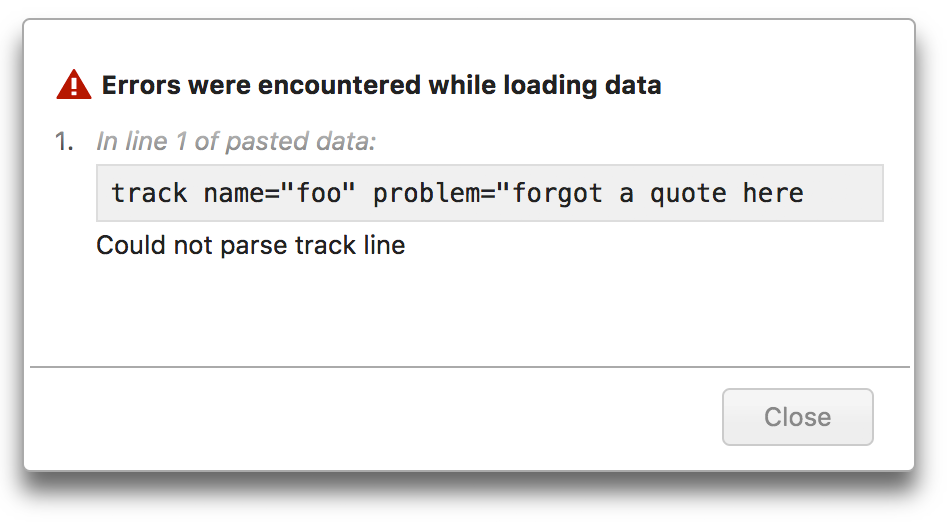
\includegraphics[width=\textwidth]{chap3/error-parsing-track}               
  \caption[Handling errors in parsing custom tracks]{If an error occurs while reading a custom track file, ChromoZoom does its best to point out to the user what went wrong, and where in the custom track file things went wrong.}
  \label{fig:error-parsing-track}
\end{marginfigure}

Despite our best intentions (and those of users providing custom track data), sometimes things go wrong while adding custom tracks to ChromoZoom. In this case, we try to generate a user-friendly message describing what the error was, and if possible, where in the file the error was encountered. A sample message is depicted in Figure \ref{fig:error-parsing-track}.

\subsection{Conclusions}

ChromoZoom v2 is the first next-generation online genome browser that supports client-side loading of custom genome assemblies along with rich annotation data. We use this new version of ChromoZoom to assess bacterial assemblies and comparative genomics analyses created as part of pathogen surveillance activities at The Mount Sinai Hospital. However, the new release of ChromoZoom is equally capable of loading standard references for vertebrate genomes and displaying the results of typical NGS experiments, such as alignments of paired-end reads from an Illumina instrument, alongside thousands of curated tracks from UCSC. We contend that ChromoZoom v2 is the first genome browser to achieve the three design goals of the user experience demonstrated by Google Maps, in that it is (1) universally accessible, (2) richly interactive, and (3) easily sharable. Assessment of NGS data continues to be an increasingly collaborative endeavor, with participants from diverse backgrounds (from bioinformatics groups to clinical staff) who are often spread across multiple institutions, even for average-sized projects. We see ChromoZoom as a platform that supports these teams.

\section*{Notes}

\subsection{Contributions}

Theodore Pak wrote the first and second versions of ChromoZoom. Miha Skalic and Adrian Pasculescu contributed to the Python pipeline for mirroring data from UCSC Genome Browser. Frederick ``Fritz'' Roth provided advice and support during the initial development of ChromoZoom and throughout the development of the second version.

\subsection{Funding}

Funding was provided by the Icahn Institute for Genomics and Multiscale Biology at Mount Sinai and NIH/NIAID (U19-AI118610 and F30-AI122673).

\subsection{Conflict of Interest}

The authors have no conflicts of interest to disclose.

\subsection{Acknowledgements}

We thank Andrew Kasarskis for supporting this project and Miguel Ranjo for providing bug reports. This work was supported in part by the resources and expertise of the Department of Scientific Computing at the Icahn School of Medicine at Mount Sinai.
